\section{Introduction}
\label{sec:intro}

We view thin curvilinear structure segmentation not as pixel-wise
classification but as the recovery of a connected network. For vessels, nerves, cracks, roads, wires,
and mortar joints, the value of a prediction is not fully captured by how many
foreground pixels it covers; whether the network remains connected is equally
important. This reveals a long-standing mismatch between evaluation and use:
two predictions with similar
Dice can differ sharply in topology---one remains usable while the other is
broken---and a single missing branch can change the outcome of a hemodynamic
simulation, a routing analysis, or a crack-propagation study. Connectivity and
topology are therefore not auxiliary metrics; they are first-class criteria on
par with overlap-based metrics \cite{shit2021cldice,kirchhoff2024skeletonrecall}.

These structures appear in fundus and OCTA images
\cite{staal2004drive,hoover2000stare,budai2013robust,li2024octa500}, coronary
angiography \cite{cervantes2019dca1}, pavement crack images
\cite{liu2019deepcrack}, aerial road imagery \cite{mnih2013machine}, and
industrial or materials imagery containing wires, tire treads, and masonry
joints \cite{zhu2026sacm,valverde2025topomortar}. They are thin, low-contrast,
and densely branched, while dense annotation is expensive and test domains
differ in modality, resolution, and acquisition conditions. Few-shot, cross-domain segmentation
is thus the central deployment challenge.

\begin{figure}[t]
\centering
\setlength{\tabcolsep}{0.6pt}
\offinterlineskip
\renewcommand{\arraystretch}{0}
\newlength{\FigOneW}\setlength{\FigOneW}{\dimexpr\columnwidth-14pt\relax}\divide\FigOneW by 4
\newlength{\FigOneLabelW}\setlength{\FigOneLabelW}{9pt}
\begin{tabular}{@{}c*{4}{c}@{}}
\makebox[\FigOneLabelW][c]{\rotatebox{90}{\scriptsize Input}} & 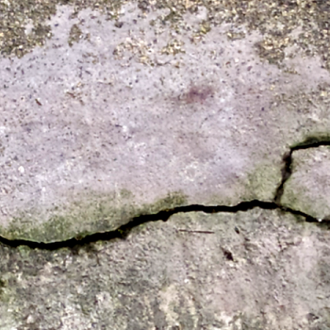
\includegraphics[width=\FigOneW]{../img/dcd_fig1/crack_raw.pdf} & 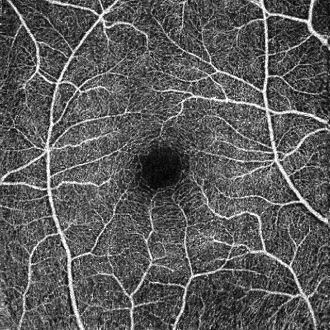
\includegraphics[width=\FigOneW]{../img/dcd_fig1/octa_raw.pdf} & 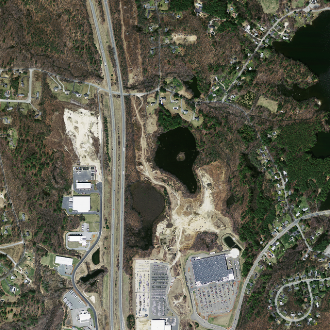
\includegraphics[width=\FigOneW]{../img/dcd_fig1/road_raw.pdf} & 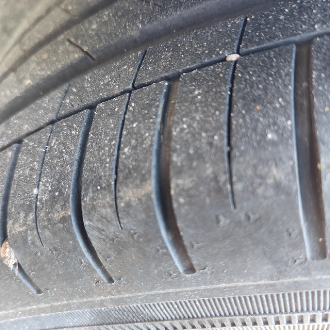
\includegraphics[width=\FigOneW]{../img/dcd_fig1/tyre_raw.pdf} \\[1pt]
\makebox[\FigOneLabelW][c]{\rotatebox{90}{\scriptsize Prediction}} & 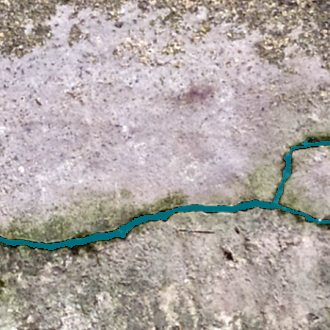
\includegraphics[width=\FigOneW]{../img/dcd_fig1/crack_ours.pdf} & 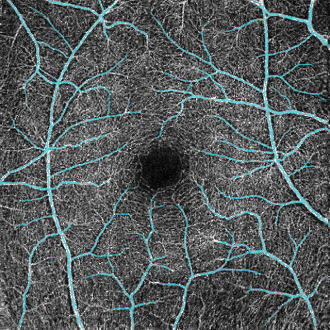
\includegraphics[width=\FigOneW]{../img/dcd_fig1/octa_ours.pdf} & 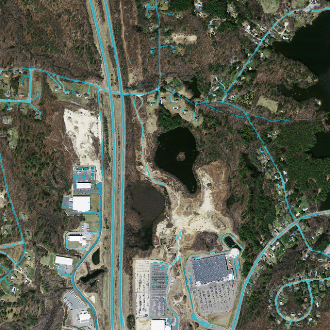
\includegraphics[width=\FigOneW]{../img/dcd_fig1/road_ours.pdf} & 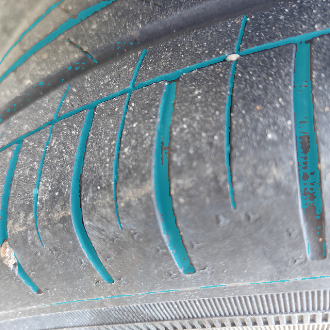
\includegraphics[width=\FigOneW]{../img/dcd_fig1/tyre_ours.pdf} \\[9pt]
\makebox[\FigOneLabelW]{} & \makebox[\FigOneW][c]{\scriptsize CHCrack5K} & \makebox[\FigOneW][c]{\scriptsize OCTA-500} & \makebox[\FigOneW][c]{\scriptsize ROAD} & \makebox[\FigOneW][c]{\scriptsize TYRE} \\
\end{tabular}
\caption{Cross-domain results of DCD. Each column shows a raw test image
(top) and the DCD prediction overlaid in cyan (bottom). Trained on only
18 images from six training datasets and deployed at a single fixed candidate
rank (slot 3), DCD preserves thin structures and connectivity on two
unseen and two novel datasets.}
\label{fig:dcd_teaser}
\end{figure}

Research has advanced along two lines. The first improves representation.
U-Net \cite{ronneberger2015unet} established the encoder--decoder template;
CS-Net \cite{mou2019csnet} and CS2-Net \cite{mou2021cs2net} introduced spatial
and channel attention to integrate local features with global dependencies;
DeepCrack \cite{liu2019deepcrack} focused on crack segmentation; and
nnWNet \cite{zhou2025nnwnet} explored transformer--convolution hybrids. The
second adds topological supervision: clDice \cite{shit2021cldice} and Skeleton
Recall \cite{kirchhoff2024skeletonrecall} incorporate skeleton or connectivity
information into the loss and alleviate fragmentation. Both lines improve
single-model performance, but both are typically developed under the
assumption that training and test data share the same distribution. Under domain shift, the confidence of a single model often
becomes unreliable. Multi-candidate decoding
offers a way to keep several complementary hypotheses before committing to one:
SAM returns multiple masks \cite{kirillov2023sam}, and SACM maintains multiple
candidate heads \cite{zhu2026sacm}.

SAM \cite{kirillov2023sam} offers a third path: a frozen ViT encoder can be
adapted with lightweight modules, enabling transfer with very few annotations.
SAM-Adapter \cite{chen2023samadapter} and Conv-LoRA \cite{zhong2024convlora}
add adapters or low-rank modules, CAT-SAM \cite{xiao2024catsam} performs
few-shot conditional tuning, and HQ-SAM \cite{ke2023hqsam} improves mask
decoding quality; UCS \cite{zhu2025ucs} adapts SAM with sparse adapters and
FFT-generated prompts, while SACM \cite{zhu2026sacm} combines dual-level
adapters with a prompt-free decoder. SACM is representative: it maintains
multiple candidate heads, ranks them by Stage-1 confidence, refines them in
Stage-2, and selects the final mask with an MLP-based IoU predictor. SACM generalizes across
12 datasets when trained on only 18 images.

This raises the central question: do the gains of multi-candidate decoding come
from generating more candidates, or from deploying them? SACM, for instance,
relies on a test-time selector \cite{zhu2026sacm}. However, the selector is
learned on the training distribution and must rank candidates on unseen
modalities; its calibration can drift, and overlap-based scores may favor
thicker, better-connected masks while discarding thin branches. One concern is
that the selector and the candidate heads are trained jointly: the heads are
encouraged to specialize, while the selector is encouraged to pick the most
stable candidate on the current distribution. This coupling may bias the
selector toward one type of candidate and cause it to neglect the other
experts. A
mechanism meant to improve robustness thus returns the final output to a
single decision point. We therefore ask: after the candidate heads
specialize, is a test-time selector still necessary? If not, can a fixed rule
replace it under domain shift?

Our starting point is simple: if the four heads are trained to take different
roles---dense, topology, boundary, and recall---then the best test-time
decision may be not to decide. We propose Deterministic Candidate Decoding
(DCD). Building on SACM's frozen SAM ViT-L, dual-level adapters, and
multi-candidate decoder, we train all four heads with dense supervision, apply
soft clDice and skeleton recall losses, and add role-specific losses to the
three auxiliary heads: an extra topology term, a boundary-weighted term, and a
recall-oriented Tversky term. A zero-initialized linear fusion serves as an
auxiliary output. At inference, gating only orders the candidates, and DCD
always deploys the last-ranked slot (slot 3), without the IoU predictor or the
fusion branch. Slot 3 is the recall-oriented Tversky expert; fixing the rank
preserves the learned role specialization while removing the selector's
per-image variability. With the same trained candidate experts, fixed deployment improves
Dice, IoU, and clDice by 1.22, 1.11, and 1.06 points over gating and fusion,
with HD95 essentially unchanged. This counterintuitive result suggests that, for this family of
decoders, the bottleneck lies in deployment rather than candidate generation.

We validate this on a strict 3-shot protocol: 18 training images from six
training datasets, 12 evaluation datasets (eight unseen and four novel
datasets), ten CNN, transformer, and SAM baselines (including two
oracle-prompted ones: SAM-OCTA and SAM-Med2D), and four seeds. DCD obtains 58.76 Dice,
45.17 IoU, 66.02 clDice, and 63.13 HD95 under a dataset-equal macro average,
ranking first on all four metrics. We also report per-dataset results and the
Dice--HD95 trade-off: DCD is not the best on every dataset, and thin-vessel cases
such as HRF and STARE expose remaining gaps. Ablations isolate the effects of
the deployment rule, role losses, topology supervision, and fusion, supporting
the deployment-bottleneck hypothesis.

Our contributions are threefold.
\begin{itemize}
\item We identify test-time candidate selection as the deployment bottleneck
of multi-candidate prompt-free decoders for thin structures, and provide
counterintuitive evidence: with the same trained candidate experts, fixed-rank deployment
improves Dice, IoU, and clDice relative to the learned selector, with
comparable HD95 and without retraining the candidate experts.
\item We propose DCD, a training-and-deployment recipe for frozen-SAM
prompt-free decoders: four candidate heads are trained with dense,
topology-aware, and role-specific supervision; at inference, gating only
orders the candidates, and DCD always deploys the last-ranked slot (slot 3),
with no IoU predictor or fusion. This turns multi-candidate decoding into a
deterministic single-output rule.
\item We follow SACM's 3-shot setting and systematically compare DCD with ten
CNN, transformer, and SAM baselines on 12 datasets (eight unseen and
four novel datasets) over four seeds; DCD ranks first on all four macro metrics.
Ablations attribute the gains mainly to role specialization and fixed
deployment, and show that the fusion auxiliary is optional.
\end{itemize}
